% !TEX program = xelatex


\documentclass{article} 
\usepackage{xltxtra} % 这个包是为了打印\XeLaTeX 的Logo。 
\usepackage{xeCJK} % 这个包可以指定中文字体。
\setCJKmainfont[Mapping=tex-text,BoldFont=SimHei]{SimSun}
\setCJKsansfont{SimHei}
\setCJKmonofont[Scale=.85]{FandolFang}
\setmainfont{Palatino Linotype}
\setmonofont{Consolas}

\usepackage{url}
\usepackage{geometry}
\geometry{left=3cm,right=3cm}

\usepackage{multirow}
\usepackage{amsfonts}

\newcommand{\e}[1]{$ \times 10^{#1}$}
\renewcommand{\figurename}{图}
\renewcommand{\tablename}{表}
\renewcommand{\today}{\number\year 年 \number\month 月 \number\day 日}

\begin{document}
 \title{Recommder System Handbook学习笔记\ 第一部分,章节5 高级协同过滤技术}
 \author{littlekideee}
 \maketitle

 \section{介绍}
 协同过滤(CF)方法基于评分或行为的模式来给用户推荐特别的项目。

 开始于2006年10月的Netflix大奖赛极大地推动了协同过滤技术的进步。这是研究团体第一次获得如此大粒度、工业级的数据集,它包含了100万电影评分。

 推荐系统依赖于各种类型的输入。最方便的类型是高度明确的反馈信息,它表达了用户对项目的直接憎恶。

 但由于明确反馈不是什么时候都可用的,一些推荐系统从大量的模糊反馈中推断用户的偏好。模糊反馈包含购买历史、浏览历史、搜索模式、甚至是鼠标轨迹。本章的模型适用于明确的反馈数据。尽管如此,我们要认识到模糊反馈的重要性,把模糊反馈作为模型中第二信息源。

 为了建立推荐系统,CF系统需要关联两个重要的实体:用户和项目。构成CF的两个主要技术为:邻域方法和潜在特征模型。邻域模型是利用用户或项目之间的相互关系来构建推荐系统地。而潜在特征模型,如矩阵分解(SVD),则是将用户和项目投影到相同的潜在特征空间中。

 预测更加准确的预测方法需要深化基础和减少对武断决策的依赖。本章描述最近CF建模技术的发展。

 \section{预备知识}
 我们给出$m$个用户(又叫做顾客),$n$个项目(又叫做产品)的评分。$r_{ui}$表示用户$u$对项目$i$的评分,这个值高表示用户对项目有更强的偏好。

 $t_{ui}$为评分$r_{ui}$的时间。我们可以根据需求使用不同的时间单元。

 数据中大部分评分时未知的。例如Netflix数据中有99\%的评分是缺失的。评分$r_{ui}$已知的$(u,i)$对被存于集合$\mathcal{K}=\{(u,i)|r_{ui}\ \mathsf{is\ known}\}$中。每个用户关联一个项目集合$R(u)$,包含了用户$u$评分过的所有项目。同样,$R(i)$表示评分过项目$i$的用户集合。有时候,我们使用集合$N(u)$来表示用户$u$产生过模糊反馈(租借、购买、查看等)的项目集合。

 \subsection{Baseline预测器}
 CF模型尝试捕捉产生不同评分的用户与项目之间的相互关系。然而,典型的CF数据中显示了很多用户和项目的偏见。

 为了中和这些影响,先排除用户-项目的相互作用,提出baseline预测器(又被叫做biases)。

 记$\mu$为全局平均评分。一个baseline预测器使用$b_{ui}$来计算未知评分$r_{ui}$,同时考虑用户和项目的影响:
 $$ b_{ui}=\mu+b_u+b_i $$

 参数$b_u$和$b_i$表明用户$u$和项目$i$的偏差。可用求解最小二乘问题来估计$b_u$和$b_i$:
 $$ \mathop{\mathsf{min}}\limits_{b_{*}}\mathop{\sum}\limits_{(u,i)\in\mathcal{K}}(r_{ui}-\mu-b_u-b_i)^2+\lambda_1(\mathop{\sum}\limits_{u}b_u^2+\mathop{\sum}\limits_{i}b_i^2) $$

 这里第一项$\mathop{\sum}_{(u,i)\in\mathcal{K}}(r_{ui}-\mu-b_u-b_i)^2$是为了找到拟合给定评分的$b_u$和$b_i$。正则项$\lambda_1(\mathop{\sum}_{u}b_u^2+\mathop{\sum}_{i}b_i^2)$是对参数惩罚以避免过拟合。求解这个最小二乘问题的算法为随机梯度下降法(SGD)。

 一个更加简单但是准确率降低的估计参数的方式:首先对每个项目$i$计算:
 $$ b_i=\frac{\mathop{\sum}_{u\in R(i)}(r_{ui}-\mu)}{\lambda_2+|R(i)|} $$

 再对每个用户$u$计算:
 $$ b_u=\frac{\mathop{\sum}_{i\in R(u)}(r_{ui}-\mu-b_i)}{\lambda_3+|R(u)|} $$

 \subsection{Netflix数据}
 为了比较本章描述的算法,我们采用的是Netflix数据集。它由超过一亿条带时间戳的99年11月到05年12月的匿名用户评分组成。评分是1到5的整数。数据集包含17770部电影,480000个用户。因此,平均而言,每部电影有5600个评分,每个用户评分数量为208。推荐结果的质量由根均方误差(RMSE)给出:
 $$ \sqrt{\mathop{\sum}\limits_{(u,i)\in TestSet}(r_{ui}-\hat{r}_{ui})^2/|TestSet|} $$

 它相对平均绝对误差而言,强调了较大的误差。

 测试集是由Netflix提供的包含140万的最近评分集。

 \subsection{模糊反馈}
 本章主要关注精确用户反馈信息,尽管如此,模糊反馈的加入对更好地理解用户行为有很大的帮助。它帮助解决数据稀疏问题。

 对Netflix数据,最自然的模糊反馈选择就是电影的租借历史,它可以给我们除了评分信息之外的用户偏好。

 \section{矩阵分解模型}
 潜在因子模型可以发现解释观测评分的潜在特征。包含pLSA、神经网络、LDA(潜在狄利克雷分配)以及哪些包含用户-项目矩阵分解的模型(也叫做基于SVD的模型)。

 将SVD应用到精确评分数据是很困难的,因为高度的缺失数据。当矩阵是不完全的时候,传统的SVD是未定义的。而且很容易过拟合。最早的解决方法是不全缺失值,但是这种方法会造成空间浪费,准确率也不好。最近的研究工作的做法是直接仅使用观测到的数据,使用充足的正则模型来避免过拟合。

 \subsection{SVD}
 矩阵分解模型将用户和项目都映射到一个维度为$f$的潜在因子空间中,用户-项目的相互作用可以建模为空间内向量的内积。潜在特征试图解释用户和产品的特征。

 每个项目$i$关联到一个向量$q_i\in\mathbb{R}^f$上,用户$u$关联到向量$p_u\in\mathbb{R}^f$上。这些向量的每个元素值都代表了用户或项目某个因子的权重。点积$q_i^Tq_u$捕捉用户$u$与项目$i$之间的关系,即用户对项目的整体兴趣。最终的评分由baseline分加这个兴趣构成:
 $$ \hat{r}_{ui}=\mu+b_i+b_u+q_i^Tq_u $$

 为了学习这个模型的参数($ b_u,b_i,p_u,q_i $),我们最小化正则平方误差:
 $$ \mathop{\mathsf{min}}\limits_{b_*,q_*,p_*}\mathop{\sum}\limits_{(u,i)\in\mathcal{K}}(r_{ui}-\mu-b_u-b_i-q_i^Tq_u)^2+\lambda_4(b_i^2+b_u^2+\|q_i\|^2+\|p_u\|^2) $$

 常量$\lambda_4$是控制正则项的参数,通过交叉验证决定。通常使用随机梯度下降和交替最小二乘法优化。

 交替最小二乘法通过$p_u$来优化$q_i$,再用$q_i$来优化$p_u$。

 随机梯度下降算法在所有训练集中评分循环。对每个给定的评分$r_{ui}$,得到一个预测$\hat{r}_{ui}$,关联的预测误差为$e_{ui}\mathop{=}\limits^{\mathsf{def}}r_{ui}-\hat{r}_{ui}$。对一个给定的训练实例$r_{ui}$,梯度方向的参数上升如下:
 \begin{itemize}
 \item $b_u\leftarrow b_u+\gamma\cdot(e_{ui}-\lambda_4\cdot b_u)$
 \item $b_i\leftarrow b_i+\gamma\cdot(e_{ui}-\lambda_4\cdot b_i)$
 \item $q_i\leftarrow q_i+\gamma\cdot(e_{ui}\cdot p_u-\lambda_4\cdot q_i)$
 \item $p_u\leftarrow p_u+\gamma\cdot(e_{ui}\cdot q_i-\lambda_4\cdot p_u)$
 \end{itemize}

 使用Netflix数据评估这个方法时,我们使用以下参数设置:$\gamma=0.005,\lambda_4=0.02$。

 \subsection{SVD++}
 还有一些方法是通过计算用户评分项目的数量来获得有意义的信息的,它通过识别那些用户评分的项目来给用户因子建模。其中我们关注SVD++。

 SVD++添加第二个项目因子集合,这个集合将每个项目$i$关联到一个因子向量$y_i\in\mathbb{R}^f$上。这些新的项目因子被用于刻画基于用户评分过的项目集合的用户。具体模型为:
 $$ \hat{r}_{ui}=\mu+b_i+b_u+q_i^T\left(p_u+|R(u)|^{-\frac{1}{2}}\mathop{\sum}\limits_{j\in R(u)}y_j\right) $$

 其中$R(u)$是用户$u$评分过的项目集合。

 现在一个用户$u$被建模为$p_u+|R(u)|^{-\frac{1}{2}}\mathop{\sum}_{j\in R(u)}y_j$。

 与SVD一样,这个模型采用随机梯度下降法优化参数:
 \begin{itemize}
 \item $b_u\leftarrow b_u+\gamma\cdot(e_{ui}-\lambda_5\cdot b_u)$
 \item $b_i\leftarrow b_i+\gamma\cdot(e_{ui}-\lambda_5\cdot b_i)$
 \item $q_i\leftarrow q_i+\gamma\cdot(e_{ui}\cdot (p_u+|R(u)|^{-\frac{1}{2}}\mathop{\sum}_{j\in R(u)}y_j)-\lambda_6\cdot q_i)$
 \item $p_u\leftarrow p_u+\gamma\cdot(e_{ui}\cdot q_i-\lambda_6\cdot p_u)$
 \item $\begin{array}{ll}
 \forall j\in R(u):\\
 y_j\leftarrow y_j+\gamma\cdot(e_{ui}\cdot|R(u)|^{-\frac{1}{2}}\cdot q_i-\lambda_6\cdot y_j)
 \end{array}
 $
 \end{itemize}

 当在Netflix数据上评估这个方法,我们使用如下的参数:$\gamma=0.007,\lambda_5=0.005,\lambda_6=0.015$。

 我们还可以使用其他类型的模糊反馈扩充到项目因子中。例如,用户$u$对项目有一个确定的偏好(如,用户租借了它们),项目集合$N^1(u)$。另外一个模糊反馈类型(例如,用户浏览了它们)的项目集合为$N^2(u)$,我们就可以使用如下模型:
 $$ \hat{r}_{ui}=\mu+b_i+b_u+q_i^T\left(p_u+|N^1(u)|^{-\frac{1}{2}}\mathop{\sum}\limits_{j\in N^1(u)}y^{(1)}_j+|N^2(u)|^{-\frac{1}{2}}\mathop{\sum}\limits_{j\in N^2(u)}y^{(2)}_j\right) $$

 每种模糊反馈的重要性通过设置相关模型参数由算法自动学习。

 \subsection{时间关联因子模型}
 我们识别下面这些在整个时间段上的影响:1)用户偏差$b_u(t)$,2)项目偏差$b_i(t)$和3)用户偏好$p_u(t)$。由于项目的特征是不会随时间变化,因此项目因子向量$q_i$还是保持静态的。

 \subsubsection{伴随时间改变的baseline预测器}
 大量的时效变化包含在baseline预测器中。第一个是项目的流行程度可能会随着时间改变,我们把$b_i$作为一个时间的函数。第二,用户会随时间改变他们baseline评分,我们把$b_u$作为一个时间的函数。这样,用户$u$对项目$i$在$t_{ui}$天,基于时间的baseline预测器为:
 $$ b_{ui}=\mu+b_u(t_{ui})+b_i(t_{ui}) $$

 其中,$b_u(\cdot)$和$b_i(\cdot)$都是时间的实值函数。这两个函数的设计应当充分考虑参数随时间变化的规律。

 在电影评分的案例中,我们不期望电影的$b_i$以‘日’为单位变化,而用户的$b_u$是以‘日’为单位变化的。

 首先从$b_i(t)$开始。我们发现可以把项目biases充分划分到基于时间的bins中,在每一个时间段使用一个项目bias常量。怎么样把时间轴划分到bins中应当平衡bins大小与每个bins中评分数量的关系。在我们的应用中,每个bin大概关联10个连续的周的数据,数据集中包含30个bins的时间段。某一天$t$关联一个整数$\mathsf{Bin}(t)$(本文的数据是一个1到30的数),则电影bias被分成一个固定的部分和一个随时间变化的部分:
 $$ b_i(t)=b_i+b_{i,\mathsf{Bin}(t)} $$

 对用户的bias来说,找到这个关于时间的函数是具有难度的。一方面我们希望对于用户找到一个短的时间段影响,另一方面,我们对每个用户又没有足够的评分来产生可信的估计。

 一个简单的建模选择使使用一个线性函数去捕捉用户bias的可能的渐近偏移。对每个用户$u$,记$t_u$为评分的平均日期。如果$u$在第$t$天评分了一个电影,那么这个评分关联的时间偏差被定义为:
 $$ \mathsf{dev}_u(t)=\mathsf{sign}(t-t_u)\cdot|t-t_u|^{\beta} $$

 其中,$|t-t_u|$度量$t$和$t_u$之间相差的天数。使用交叉验证来确定参数$\beta$,我们的应用中$\beta=0.4$。我们介绍一个新的参数,$\alpha_u$,由此我们得到第一个依赖时间的用户bias:
 $$ b_u^{(1)}(t)=b_u+\alpha_u\cdot\mathsf{dev}_u(t) $$

 一个更加灵活的参数由样条插值得到。令$u$为关联到$n_u$个评分的用户。我们设计一个$k_u$个时间点,$\{t_1^u,\dots,t_{k_u}^u\}$,这些点是均匀的,由此得到:
 $$ b_u^{(2)}(t)=b_u+\frac{\mathop{\sum}_{l=1}^{k_u}e^{-\sigma|t-t_l^u|}b_{t_l}^u}{\mathop{\sum}_{l=1}^{k_u}e^{-\sigma|t-t_l^u|}} $$

 参数$b_{t_l}^u$关联一个控制点,自动从数据中学习得到。控制点的数量$k_u$需要平衡灵活度与计算效率。本文设置$k_u=b_u^{0.25}$。常量$\sigma$的作用是平滑样条曲线,通过交叉验证我们设置$\sigma=0.3$。

 在某些情况下,在单个某天用户的bias可能会突然产生偏移。例如,在电影数据中,我们发现用户在单天内给出的多数评分都趋于固定在一个值附近。为了解决这个短期效应,我们设计了一个参数,$b_{u,t}$,用来表示特定天的变化。

 在Netflix电影数据集中,每个用户平均有40天的评分。因此,根据$b_{u,t}$的需求,平均而言,描述每个用户bias的参数有40个。则加入了$b_{u,t}$的时间线性变为:
 $$ b_u^{(3)}(t)=b_u+\alpha_u\cdot\mathsf{dev}_u(t)+b_{u,t} $$

 同样的,基于样条的模型变为:
 $$ b_u^{(4)}(t)=b_u+\frac{\mathop{\sum}_{l=1}^{k_u}e^{-\sigma|t-t_l^u|}b_{t_l}^u}{\mathop{\sum}_{l=1}^{k_u}e^{-\sigma|t-t_l^u|}}+b_{u,t} $$

 由于无视了用户与项目之间的相互作用,一个baseline预测器是无法生成个性化的推荐的。但尽管如此,加入了时序概念的预测器还是比标准预测器的误差要优秀的。为了学习参数我们通过SGD最小化带正则项的平方误差。例如,采取时间线性模型baseline预测器:
 $$ b_{ui}=\mu+b_u+\alpha_u\cdot\mathsf{dev}_u(t_{ui})+b_{u,t_{ui}}+b_i+b_{i,\mathsf{Bin}(t_{ui})} $$

 学习相关参数,$b_u,\alpha_u,b_{u,t},b_i,b_{i,\mathsf{Bin}(t)}$,的方法是,解决如下最优化问题:
 \[ 
 \begin{array}{c}
 \mathsf{min}\mathop{\sum}\limits_{(u,i)\in\mathcal{K}}(r_{ui}-\mu-b_u-\alpha_u\cdot\mathsf{dev}_u(t_{ui})-b_{u,t_{ui}}-b_i-b_{i,\mathsf{Bin}(t_{ui})})^2\\
 +\lambda_7(b_u^2+\alpha_u^2+b_{u,t_{ui}}^2+b_i^2+b_{i,\mathsf{Bin}(t_{ui})}^2) 
 \end{array}
 \]

 \begin{table}[!htb]\label{table1}
 \centering
 \caption{baseline预测器对比。加入了时序的模型变得更加准确(较小的RMSE值)}
 \begin{tabular}{c|c|c|c|c|c|c}
 	\textbf{model} & static & mov & linear & spline & linear+ & spline+ \\\hline
 	\textbf{RMSE} & .9799 & .9771 & .9731 & .9714 & .9605 & .9603 
 \end{tabular}
 \end{table}

 表1比较了加入时序前后模型RMSE值的变化。我们对每个模型的设置如下:
 \begin{itemize}
 \item static:$ b_{ui}=\mu+b_u+b_i $
 \item mov:$ b_{ui}=\mu+b_u+b_i+b_{i,\mathsf{BIN}(t_{ui})} $
 \item linear:$b_{ui}=\mu+b_u+\alpha_u\cdot\mathsf{dev}_u(t_{ui})+b_i+b_{i,\mathsf{Bin}(t_{ui})}$
 \item spline:$b_{ui}=\mu+b_u+\frac{\mathop{\sum}_{l=1}^{k_u}e^{-\sigma|t-t_l^u|}b_{t_l}^u}{\mathop{\sum}_{l=1}^{k_u}e^{-\sigma|t-t_l^u|}}+b_i+b_{i,\mathsf{Bin}(t_{ui})}$
 \item linear+:$ b_{ui}=\mu+b_u+\alpha_u\cdot\mathsf{dev}_u(t_{ui})+b_{u,t_{ui}}+b_i+b_{i,\mathsf{Bin}(t_{ui})} $
 \item spline+:$ b_{ui}=\mu+b_u+\frac{\mathop{\sum}_{l=1}^{k_u}e^{-\sigma|t-t_l^u|}b_{t_l}^u}{\mathop{\sum}_{l=1}^{k_u}e^{-\sigma|t-t_l^u|}}+b_{u,t_{ui}}+b_i+b_{i,\mathsf{Bin}(t_{ui})}$
 \end{itemize}

 除了以上方法描述的时间效应的影响以外,还有一些其他方面的影响。比如说捕捉定期(periodic)影响。例如,某些产品可能在特定的季节或假期比其他时间更加流行。定期影响也可以在用户这边找到,比如用户在周末和工作日的购买模式是不同的。建模这种定期影响的方法是采用一个参数来表示时间段内项目或用户的bias。由此,项目bias变成:
 $$ b_i(t)=b_i+b_{i,\mathsf{Bin}(t)}+b_{i,\mathsf{period}(t)} $$

 例如,我们如果想找到项目bias在一年四季中的变化,那么令$period(t)\in\{fall,winter,spring,summer\}$即可。同样的,用户bias则变为:
 $$ b_u(t)=b_u+\alpha_u\cdot\mathsf{dev}_u(t)+b_{u,t}+b_{u,\mathsf{period}(t)} $$

 然而在电影评分数据集中,这种定期影响没有什么意义。

 除此之外,用户评分尺度也会随着时间而变化。因此,我们添加一个依赖时间的尺度特征到baseline预测器中,记为$c_u(t)$。则baseline预测器变为:
 $$ b_{ui}=\mu+b_u+\alpha_u\cdot\mathsf{dev}_u(t_{ui})+b_{u,t_{ui}}+(b_i+b_{i,\mathsf{Bin}(t_{ui})})\cdot c_u(t_{ui}) $$

 \subsubsection{时间变化的因子模型}
 除了上小节的baseline中的用户项目bias会随时间变化之外,用户的品位也会随时间变化。即表示用户的向量$p_u$是关于时间的一个函数。事实上,时间对用品偏好的影响是非常难以捕捉的,因为不像用户bias,$p_u$是有许多因子组成的。

 我们将用户偏好的每一个成分都加以建模$p_u(t)^T=(p_{u1}(t),\dots,p_{uf}(t))$。在电影评分数据集中,我们将用户偏好建模为;
 $$ p_{uk}(t)=p_{uk}+\alpha_{uk}\cdot\mathsf{dev}_u(t)+p_{uk,t}\quad k=1,\dots,f $$

 由此,我们可以扩展SVD++模型为\textit{timeSVD++}:
 $$ \hat{r}_{ui}=\mu+b_i(t_{ui})+b_u(t_{ui})+q_i^T\left(p_u(t_{ui})+|R(u)|^{-\frac{1}{2}}\mathop{\sum}\limits_{j\in R(u)}y_j\right) $$

 使用SGD优化参数。

 \subsection{比较}
 表2比较了本节中所讨论的三个算法的实验结果。

 \begin{table}[!htb]
 \centering
 \caption{三个因子模型的比较:RMSE随着维度$f$的变化。对所有的模型,RMSE随着$f$的增多而减小。timeSVD++比SVD++较好,而SVD++又比原始的SVD效果要好。}
 \begin{tabular}{|l|c|c|c|c|c|}\hline
 Model & $f=10$ & $f=20$ & $f=50$ & $f=100$ & $f=200$ \\\hline
 SVD & .9140 & .9074 & .9046 & .9025 & .9009 \\
 SVD++ & .9131 & .9032 & .8952 & .8924 & .8911 \\
 timeSVD++ & .8971 & .8891 & .8824 & .8805 & .8799 \\\hline
 \end{tabular}
 \end{table}

 \subsubsection{未来时间的预测}
 我们怎样预测未来的评分?一个简单的方法就是对未来的数据,特定天参数应该取默认值。$c_u(t_{ui})$设置为$c_u$,$b_{u,t_{ui}}$设置为零。

 \section{邻域模型}
 大多数CF方法都是基于邻域模型的。先是基于用户,再到基于项目。虽然潜在因子模型可以给出更高的预测准确度,但是现实系统还是采用邻域方法较多,原因是邻域方法产生的结果高度可解释而且邻域方法的扩展性也较好。

 \subsection{相似度度量}
 基于项目方法的相似度度量一般基于Pearson相关系数,$\rho_{ij}$。由于很多评分是未知的,一些项目只有少量的共同评分用户。经验相关系数,$\hat{\rho}_{ij}$仅基于共同用户计算。
 $$ \hat{\rho}_{ij}=\frac{\sum_{u\in U(i,j)}(r_{ui}-b_{ui})(r_{uj}-b_{uj})}{\sqrt{\sum_{u\in U(i,j)}(r_{ui}-b_{ui})^2\cdot\sum_{u\in U(i,j)}(r_{uj}-b_{uj})^2}} $$

 集合$U(i,j)$包含了既评分了$i$又评分了$j$的用户集合。$b$为baseline预测器。

 因为估计关联系数在支持用户数越多的情况下越可靠,一种更合适的度量方法为:
 $$ s_{ij}\mathop{=}\limits^{def}\frac{n_{ij}-1}{n_{ij}-1+\lambda_8}\rho_{ij} $$

 变量$n_{ij}=|U(i,j)|$。一般取$\lambda_8=100$。

 \subsection{基于相似度的插值}
 使用相似度方法,我们找出用户$u$评分过的与$i$最相似的$k$个项目。这$k$个邻居的集合记为$S^k(i;u)$。预测评分由计算邻居的加权平均评分计算:
 $$ \hat{r}_{ui}=b_{ui}+\frac{\sum_{j\in S^k(i;u)}s_{ij}(r_{uj}-b_{uj})}{\sum_{j\in S^k(i;u)}s_{ij}} $$

 有时候,将相似度转化为一些其他权重会产生更好的结果。例如,有些数据集上使用相似度的平方更好:$\hat{r}_{ui}=b_{ui}+\frac{\sum_{j\in S^k(i;u)}s_{ij}^2(r_{uj}-b_{uj})}{\sum_{j\in S^k(i;u)}s_{ij}^2}$。

 基于相似度的方法因为它的直观且易于应用变得非常流行。它们还提供以下两个有用的属性:
 \begin{enumerate}
 \item 可解释性。
 \item 实时性。新加入的评分可以立即将系统更新。
 \end{enumerate}

 然而,标准的基于邻域方法也产生了一些问题:
 \begin{enumerate}
 \item 相似度函数($s_{ij}$)是arbitrary。
 \item 这些方法没有考虑邻居之间的交互关系。
 \item 由定义,插值权重和为1,这可能导致过拟合。
 \item 邻域方法可能当邻居评分有明显变化时可能失效。
 \end{enumerate}

 这些问题都可以使用一些方法控制。例如第三个,可以加一个sum-to-one约束:
 $$ \hat{r}_{ui}=b_{ui}+\frac{\sum_{j\in S^k(i;u)}s_{ij}(r_{uj}-b_{uj})}{\lambda_9+\sum_{j\in S^k(i;u)}s_{ij}} $$

 $\lambda_9$可以在当没有邻域信息时(即$\sum_{j\in S^k(i;u)}s_{ij}<<\lambda_9$)惩罚邻域划分。

 \subsection{联合导出插值权重}
 给出1邻域集合$S^k(i;u)$,我们需要计算插值权重$\{\theta_{ij}^u|j\in S^k(i;u)\}$,它能产生最好的预测:
 $$ \hat{r}_{ui}=b_{ui}+\mathop{\sum}\limits_{j\in S^k(i;u)}\theta_{ij}^u(r_{uj}-b_{uj}) $$

 邻居数量$k$一般取20-50之间。定义残差评分$z_{ui}\mathop{=}\limits^{def}r_{ui}-b_{ui}$。并且为了方便,将$S^k(i;u)$中的项目从$1,\dots,k$编号。

 \subsubsection{正式模型}
 我们先考虑除了用户$u$,其他所有用户都评分了$i$和它所有的邻居$S^k(i;u)$。在这种情况下,我们可以使用最小二乘法学习插值权重:
 $$ \mathop{\mathsf{min}}\limits_{\theta^u}\mathop{\sum}\limits_{v\neq u}\left(z_{vi}-\mathop{\sum}\limits_{j\in S^k(i;u)}\theta_{ij}^uz_{vj}\right)^2 $$

 从统计学角度来看,它等同于一个$z_{vi}$在$j\in S^k(i;u)$的$z_{vj}$上做线性回归的结果。最优的权重由:
 $$ Aw=b $$

 给出。这里,$w\in\mathbb{R}^k$是未知的向量,$w_j$代表系数$\theta_{ij}^u$。$A$是一个$k\times k$的矩阵,定义为;
 $$ A_{jl}=\mathop{\sum}\limits_{v\neq u}z_{vj}z_{vl} $$

 相似的,向量$b\in\mathbb{R}^k$定义为:
 $$ b_j=\mathop{\sum}\limits_{v\neq u}z_{vj}z_{vi} $$

 由于评分矩阵的稀疏性,由以上两个式子计算$A$和$b$是不明智的。我们可以通过一下方式来估计$A$和$b$:
 $$ \bar{A}_{jl}=\frac{\sum_{v\in U(j,l)}z_{vj}z_{vl}}{|U(j,l)|} $$
 $$ \bar{b}_{j}=\frac{\sum_{v\in U(i,j)}z_{vj}z_{vi}}{|U(i,j)|} $$

 这仍然没有克服稀疏的问题。根据之前的讨论,支持度较小($|U(i,j)|$很小)的均值可以通过收缩到一个共同的值来提升。特定地,我们计算所有可能的$\bar{A}_{jl}$的均值来定义一个baseline值。记做$avg$。据此,将$k\times k$矩阵$\hat{A}$和向量$\hat{b}\in\mathbb{R}^k$定义为:
 $$ \hat{A}_{jl}=\frac{|U(j,l)|\cdot\bar{A}_{jl}+\beta\cdot avg}{|U(j,l)|+\beta} $$
 $$ \hat{b}_{j}=\frac{|U(i,j)|\cdot\bar{b}_{j}+\beta\cdot avg}{|U(i,j)|+\beta} $$

 参数$\beta$为收缩的程度,典型的取值为$\beta=500$。

 关于$A$和$b$最好的估计就是$\hat{A}$和$\hat{b}$。我们可以通过求解$\hat{A}w=\hat{b}$得到最优的插值权重,从而可以计算预测分$r_{ui}$。

 \subsubsection{计算问题}
 基于项目的邻域方法的计算效率需要预计算一些关联每个项目-项目对的值。首先,我们需要预先计算左右项目之间的相似度$s_{ij}$。

 第二,我们需要预计算所有$\hat{A}$和$\hat{b}$的可能项。对每两个项目$i$和$j$,我们计算:
 $$ \bar{A}_{ij}=\frac{\sum_{v\in U(i,j)}z_{vi}z_{vj}}{|U(i,j)|} $$

 $avg$的值取提前计算的$n\times n$矩阵的$\bar{A}$的均值。

\section{丰富邻域模型}
与矩阵分解不同,大多数邻域方法都是本地的,仅仅关注评分的一小部分子集。本节的目的是采用全局的观点来提升预测准确度。

\subsection{一个全局的邻域模型}
\subsubsection{建立模型}
$j$到$i$的权重记为$w_{ij}$,通过最优化学习得到。模型初始的框架将每个评分$r_{ui}$描述为:
$$ \hat{r}=b_{ui}+\mathop{\sum}\limits_{j\in R(u)}(r_{uj}-b_{uj})w_{ij} $$

这里我们不再把权重解释为插值系数,而认为其是调节参数,或加到baseline预测器上的偏移量。

我们可以使用二元形式的用户输入。即,不管评分值,仅分析那个项目被评分。增加另一个权重集,将评分重写为:
$$ \hat{r}=b_{ui}+\mathop{\sum}\limits_{j\in R(u)}[(r_{uj}-b_{uj})w_{ij}+c_{ij}] $$

我们将会使用另一个隐式反馈集合,$N(u)$,评分变为:
$$ \hat{r}=b_{ui}+\mathop{\sum}\limits_{j\in R(u)}(r_{uj}-b_{uj})w_{ij}+\mathop{\sum}\limits_{j\in N(u)}c_{ij} $$

引用全局权重来代替特定用户的系数是为了强调未知评分的影响,换句话说,一个用户的观点不仅仅由他的评分形成,还会受他未评分的项目影响。

我们可以将$b_{ui}$和$b_{uj}$的定义分离开来。因此,更加一般的预测规则将变为:$\hat{r}=\tilde{b}_{ui}+\mathop{\sum}_{j\in R(u)}(r_{uj}-b_{uj})w_{ij}+c_{ij}$。常数$\tilde{b}_{ui}$可以使用其他模型对$r_{ui}$的预测。这里建议使用以下规则,它的表现很好。
$$ \hat{r}=\mu+b_u+b_i+\mathop{\sum}\limits_{j\in R(u)}[(r_{uj}-b_{uj})w_{ij}+c_{ij}] $$

我们还发现对求和归一化对模型是有提升的:
$$ \hat{r}=\mu+b_u+b_i+|R(u)|^{-\alpha}\mathop{\sum}\limits_{j\in R(u)}[(r_{uj}-b_{uj})w_{ij}+c_{ij}] $$

$\alpha$常量控制归一化的强度。我们希望,如果用户评分较多,预测分应当尽量偏离baseline,反之,预测分应当接近baseline。在Netflix上的实验表明,当$\alpha=0.5$时,结果最好:
$$ \hat{r}=\mu+b_u+b_i+|R(u)|^{-\frac{1}{2}}\mathop{\sum}\limits_{j\in R(u)}[(r_{uj}-b_{uj})w_{ij}+c_{ij}] $$

为了减少模型的复杂度,我们可以将参数中关于项目之间相似度较低的去掉。记$S^k(i)$为与$i$相似的前$k$和项目的集合。使用$R^k(i;u)\mathop{=}\limits^{def}R(u)\cap S^k(i)$。则预测分变为:
$$ \hat{r}=\mu+b_u+b_i+|R^k(i;u)|^{-\frac{1}{2}}\mathop{\sum}\limits_{j\in R^k(i;u)}[(r_{uj}-b_{uj})w_{ij}+c_{ij}] $$

\subsubsection{参数估计}
上节的模型非常适合快速在线预测。新模型的主要设计目标有效全局优化过程。因此,模型参数通过解决正则化的最小二乘问题学习:
\[ 
\begin{array}{ccl}
\mathop{\mathsf{min}}\limits_{b_*,w_*,c_*} & \mathop{\sum}\limits_{(u,i)\in\mathcal{K}} & \left(r_{ui}-\mu-b_u-b_i-|R^k(i;u)|^{-\frac{1}{2}}\mathop{\sum}\limits_{j\in R^k(i;u)}((r_{uj}-b_{uj})w_{ij}+c_{ij})\right)^2\\
& & +\lambda_{10}\left(b_u^2+b_i^2+\mathop{\sum}\limits_{j\in R^k(i;u)}w_{ij}^2+c_{ij}\right) 
\end{array}
\]

我们发现简单随机梯度下降法非常快。记预测误差,$r_{ui}-\hat{r}_{ui}$,为$e_{ui}$。在所有已知评分$\mathcal{K}$内循环。对一个给定的训练实例$r_{ui}$,我们通过移动与梯度相反的方向来修改参数:
\begin{itemize}
\item $b_u\leftarrow b_u+\gamma\cdot(e_{ui}-\lambda_{10}\cdot b_u)$
\item $b_i\leftarrow b_i+\gamma\cdot(e_{ui}-\lambda_{10}\cdot b_i)$
\item $\forall j\in R^k(i;u):$

$w_{ij}\leftarrow w_{ij}+\gamma\cdot\left(|R^k(i;u)|^{-\frac{1}{2}}\cdot e_{ui}\cdot(r_{uj}-b_{uj})-\lambda_{10}\cdot w_{ij}\right)$

$c_{ij}\leftarrow c_{ij}+\gamma\cdot\left(|R^k(i;u)|^{-\frac{1}{2}}\cdot e_{ui}-\lambda_{10}\cdot c_{ij}\right)$
\end{itemize}

参数$\gamma$和$\lambda_{10}$通过交叉验证获得。对Netflix数据集,取$\gamma=0.005,\lambda_{10}=0.002$。$k$值代表选择的邻域中项目数量,它的取值一般要在预测准确度和计算复杂度之间衡量。

取极限值$k=\infty$时,模型训练的计算复杂度为$O(\sum_{u}|R(u)|^2)$。

\subsubsection{准确度比较}
实验数据:Netflix数据集。

实验模型:全局优化邻域模型,简写为GlobalNgbr。

实验标准:RMSE,每次迭代时间。

比较模型:1.基于相似度的邻域模型(4.2),简记为CorNgbr,2.4.3中描述的更加准确的模型,简记为JointNgbr。

\begin{figure}[htb]
	\centering
	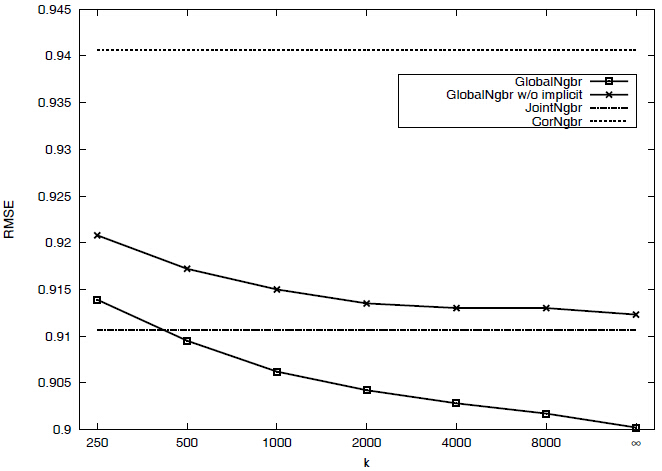
\includegraphics[scale=0.6]{f1.jpg}
	\caption{基于邻域模型的比较。}
\end{figure}

\begin{figure}[htb]
	\centering
	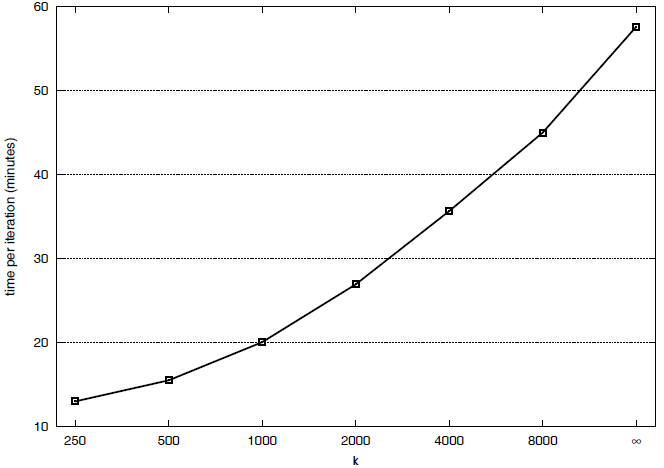
\includegraphics[scale=0.6]{f2.jpg}
	\caption{全局优化邻域模型随着参数$k$变化,迭代时间的变化。}
\end{figure}

\subsubsection{因子化项目-项目关系}
我们将每个项目$i$关联到三个向量:$q_i,x_i,y_i\in\mathbb{R}^f$。将$w_{ij}$限制为$q_i^Tx_i$,$c_{ij}=q_i^Ty_j$。将这些带入到之前的公式中得到以下预测规则:
$$ \hat{r}_{ui}=\mu+b_u+b_i+|R(u)|^{-\frac{1}{2}}\mathop{\sum}\limits_{j\in R(u)}[(r_{uj}-b_{uj})q_i^Tx_j+q_i^Ty_j] $$

提取一个$q_i^T$使计算收益更明显:
$$ \hat{r}_{ui}=\mu+b_u+b_i+q_i^T\left(|R(u)|^{-\frac{1}{2}}\mathop{\sum}\limits_{j\in R(u)}(r_{uj}-b_{uj})x_j+y_j\right) $$

一般地,我们最小化正则平方误差函数来学习参数:
\[ 
\begin{array}{ccl}
\mathop{\mathsf{min}}\limits_{q_*,x_*,y_*,b_*} & \mathop{\sum}\limits_{(u,i)\in\mathcal{K}} & \left(r_{ui}-\mu-b_u-b_i-q_i^T\left(|R(u)|^{-\frac{1}{2}}\mathop{\sum}\limits_{j\in R(u)}(r_{uj}-b_{uj})x_j+y_j\right)\right)^2\\
& & +\lambda_{11}\left(b_u^2+b_i^2+\|q_i\|^2+\mathop{\sum}\limits_{j\in R(u)}\|x_j\|^2+\|y_j\|^2\right) 
\end{array}
\]

使用下图的随机梯度法来优化参数:
\begin{figure}[htb]
	\centering
	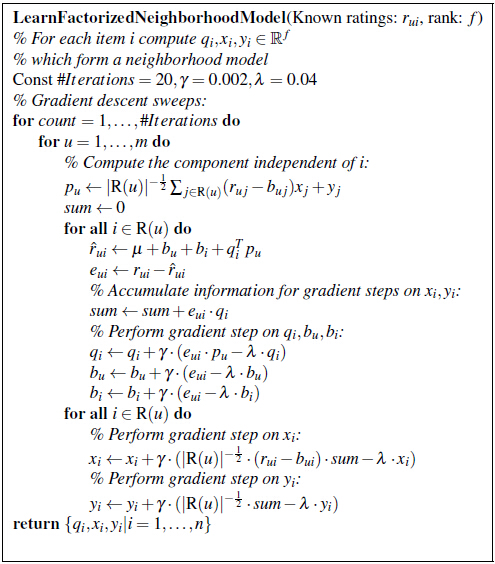
\includegraphics[scale=0.6]{f3.jpg}
\end{figure}

这个模型的时间复杂度是关于输入线性的,$O(f\cdot\sum_u(|R(u)|))$。在Netflix数据集上的实验结果由表3给出。
\begin{table}[htb]
\centering
\caption{因子化的项目-项目邻域模型的表现。因子$\geq 200$的模型是比非因子化模型表现好的,而且他的运行时间还短。}
\begin{tabular}{|l|c|c|c|c|}\hline
\# factors & 50 & 100 & 200 & 500 \\\hline
RMSE & 0.9037 & 0.9013 & 0.9000 & 0.8998 \\\hline
time/iteration & 4.5 min & 8 min & 14 min & 34 min \\\hline
\end{tabular}
\end{table}

因子化模型还有一个优势是减少空间复杂度到线性。

这个模型与一些潜在因子模型很相似。主要区别本节模型因子化项目-项目关系而不是评分本身。这个模型效果与SVD差不多的,但比SVD++要差。相比SVD,这个模型的优势在于其可解释性与对新的评分的实时影响。

\subsubsection{一个用户-用户模型}
与项目-项目模型相似,用户-用户模型考虑用户之间的关系。将之前的项目关系$w_{ij}$权重替换为用户的权重,得到评分:
$$ \hat{r}_{ui}=\mu+b_u+b_i+|R(i)|^{-\frac{1}{2}}\mathop{\sum}\limits_{v\in R(i)}(r_{vi}-b_{vi})w_{uv} $$

集合$R(i)$包含所有评分了$i$的用户。这里没有加隐式反馈的原因是我们发现在Netflix数据上没什么提升。

用户-用户模型在某些场景下是十分有用的。比如,一个系统中,项目迭代更新很快。

这个模型主要的缺点是计算复杂度高。

\paragraph{因子化模型}
计算复杂度问题可以通过与项目-项目模型中的一样的想法解决。将每个用户$u$关联到两个向量$p_u,z_u\in\mathbb{R}^f$上。假设用户-用户关系为$w_{uv}=p_u^Tz_v$。带入评分公式得:
$$ \hat{r}_{ui}=\mu+b_u+b_i+|R(i)|^{-\frac{1}{2}}\mathop{\sum}\limits_{v\in R(i)}(r_{vi}-b_{vi})p_u^Tz_v $$

同样地,为了计算效率考虑,将独立于$u$的项从求和项中提出;
$$ \hat{r}_{ui}=\mu+b_u+b_i+p_u^T|R(i)|^{-\frac{1}{2}}\mathop{\sum}\limits_{v\in R(i)}(r_{vi}-b_{vi})z_v $$

实验结果如表4所示。
\begin{table}[htb]
\centering
\caption{因子化的用户-用户邻域模型的表现。}
\begin{tabular}{|l|c|c|c|c|}\hline
\# factors & 50 & 100 & 200 & 500 \\\hline
RMSE & 0.9119 & 0.9110 & 0.9101 & 0.9093 \\\hline
time/iteration & 3 min & 5 min & 8.5 min & 18 min \\\hline
\end{tabular}
\end{table}

\paragraph{融合项目和用户模型}
本文的方法是在训练阶段就把两个模型联合起来。
\[ 
\begin{array}{cl}
\hat{r}_{ui}= & \mu+b_u+b_i+|R(u)|^{-\frac{1}{2}}\mathop{\sum}\limits_{j\in R(u)}[(r_{uj}-b_{uj})q_i^Tx_j+q_i^Ty_j]\\
&  +|R(i)|^{-\frac{1}{2}}\mathop{\sum}\limits_{v\in R(i)}(r_{vi}-b_{vi})p_u^Tz_v 
\end{array}
\]

参数学习与之前的类似。实践结果表明比单模型的表现要好,例如100个factor,RMSE值为0.8966,200个factor,RMSE0.8953。

\subsection{邻域模型中的动态时序}
将之前的评分分为两个部分,第一,$\mu+b_i+b_u$,baseline预测器,这个在之前的小节中讨论过如何增加时序。第二个,$|R(u)|^{-\frac{1}{2}}\mathop{\sum}{j\in R(u)}(r_{uj}-b_{uj})w_{ij}+c_{ij}$,这个部分,通过处理用户-项目的相互关系,可以捕捉更多信息。

项目-项目权重($w_{ij}$和$c_{ij}$)随时间是固定不变的。但是在计算权重的时候,权值可能会受到用户口味变化的影响。例如用户给$i$和$j$都打了高分,这两个项目的$w_{ij}$值应当很大,但是如果用户打分时间间隔了5年,用户的口味可能已经改变,权重值就不能确定了。

我们的目标是排除时间的干扰,得到项目-项目权重更加准确的值。首先,我们需要参数化$u$评分的两个项目之间的衰变关系。使用一个衰变函数$e^{-\beta_u\cdot\Delta t}$,其中$\beta_u>0$控制特定用户的衰变率,可以从数据中学习得到。当然,还有其他的一些衰变形式,如计算友好的$(1+\beta_u\Delta t)^{-1}$,它的结果一样,但是运行时间较快。

那么,预测规则变为:
$$ \hat{r}_{ui}=\mu+b_i(t_{ui})+b_u(t_{ui})+|R(u)|^{-\frac{1}{2}}\mathop{\sum}\limits_{j\in R(u)}e^{-\beta_u\cdot|t_{ui}-t_{uj}|}((r_{uj}-b_{uj})w_{ij}+c_{ij}) $$

相关参数,$b_i(t_{ui})=b_i+b_{i,Bin(t_{ui})}$,$b_u(t_{ui})=b_u+\alpha_u\cdot dev_u(t_{ui})+b_{u,t_{ui}}$,$\beta_u$,$w_{ij}$,$c_{ij}$,通过最小化正则化的平方误差学习:
\[ 
\begin{array}{cl}
\mathop{\sum}\limits_{(u,i)\in\mathcal{K}} & \left(r_{ui}-\mu-b_i-b_{i,Bin(t_{ui})}-b_u-\alpha_u dev_u(t_{ui})-b_{u,t_{ui}}-\right.\\
  & \left.|R(u)|^{-\frac{1}{2}}\mathop{\sum}\limits_{j\in R(u)}e^{-\beta_u\cdot|t_{ui}-t_{uj}|}((r_{uj}-b_{uj})w_{ij}+c_{ij})\right)^2+\\
  & \lambda_{12}\left(b_i^2+b_{i,Bin(t_{ui})}^2+b_u^2+\alpha_u^2+b_{u,t}^2+w_{ij}^2+c_{ij}^2\right)
\end{array}
\]

实验过程:25次迭代,$\lambda_{12}=0.002$,学习率为0.005。在学习$\beta_u$时使用了非常小的学习率$10^{-7}$。

我们希望指出一个有趣的点。假设用户$u$的偏好变化很快($\beta_u$很大)。那么,$u$老的评分应该不会很影响他现在的状态。
\[
\begin{array}{cl}
\mathop{\sum}\limits_{(u,i)\in\mathcal{K}}e^{-\beta_u\cdot|t_{ui}-t_{uj}|} & \left(r_{ui}-\mu-b_i-b_{i,Bin(t_{ui})}-b_u-\alpha_u dev_u(t_{ui})-\right.\\
  & \left.b_{u,t_{ui}}-|R(u)|^{-\frac{1}{2}}\mathop{\sum}\limits_{j\in R(u)}((r_{uj}-b_{uj})w_{ij}+c_{ij})\right)^2+\lambda_{12}(\cdot\cdot\cdot)
\end{array}
\]

这个损失函数仅关注用户当时的状态(在时间$t$)。

\section{邻域与分解}
本章一个描述了两种不同的CF方法:分解法和邻域法。每个方法都基于不同的原则,导向了不同的预测规则。需要指出,分解法会产生较好的准确率,而邻域方法有一些实践上的优点。本节将展示两者的共同之处,毕竟,他们都是线性模型。

先考虑SVD模型,它基于
$$ \hat{r}_{ui}=q_i^Tp_u $$

我们及所有项目因子为$n\times f$的矩阵$Q=[q_1q_2\dots q_n]^T$。用户因子为$m\times f$的矩阵$P=[p_1p_2\dots p_n]^T$。使用$n_u\times f$矩阵$Q[u]$约束用户$u$评论过的项目因子矩阵,其中$n_u=|R(u)|$。令向量$r_u\in\mathbb{R}^{n_u}$包含了由用户$u$给出的$Q[u]$中的有序评分。现在我们可以记录一个评分的矩阵形式,来记录所有来自$u$的评分:
$$ \hat{r}_{u}=Q[u]p_u $$

$Q[u]$固定,$\|r_u-Q[u]p_u\|_2$由下式最小化:
$$ p_u=(Q[u]^TQ[u])^{-1}Q[u]^Tr_u $$

实践中,我们加入正则项,$\lambda>0$,得到
$$ p_u=(Q[u]^TQ[u]+\lambda I)^{-1}Q[u]^Tr_u $$

将上式带入到原式中,得:
$$ \hat{r}_{ui}=Q[u](Q[u]^TQ[u]+\lambda I)^{-1}Q[u]^Tr_u $$

记$f\times f$矩阵$(Q[u]^TQ[u]+\lambda I)^{-1}$为$W^u$,可以被认为关联到用户$u$的一个权重矩阵。相应的,来自用户$u$观点的项目$i$和$j$之间的相似度可记为$s^u_{ij}^u=q_i^TW^uq_j$。使用这些新的记号,可以将SVD的预测重写为:
$$ \hat{r}_{ui}=\mathop{\sum}\limits_{j\in R(u)}s_{ij}^ur_{uj} $$

这样,我们就将SVD模型简化为一个线性模型。这个模型等价于邻域模型。我们将矩阵分解转化为项目-项目模型,转化的特点为:
\begin{itemize}
\item 插值由所有过去的用户评分得到,不仅仅是那些与项目相似的项目评分。
\item 项目$i$和$j$的相关性被分解为两个向量的内积。
\item 项目-项目权重受特定用户归一化,通过矩阵$W^u$。
\end{itemize}

\end{document}